\section{Results}
\label{sec:Results}

% The anomaly detection system achieved strong performance in identifying anomalous audio recordings of Slide Rail machines. Using a reconstruction error-based approach, the CAE model achieved the following metrics using a threshold of 0.12 determined through F1 optimization:

The proposed anomaly–detection pipeline attains competitive performance on the Slide-Rail subset of the ToyADMOS2 benchmark. Table \ref{tab:cae_vs_svdd} summarises the main quantitative findings, while Figure \ref{fig:Accuracy and loss plot} and \ref{fig:Reconstructed error plot} provide diagnostic visualisations that underpin our discussion.


% \begin{table}[H]
% \center
% \caption{Achieved metrics of model performance.}
% \begin{tabular}{l|l}
% \textbf{Metric}   & \textbf{Value} \\ \hline
%  Precision & 0.8864 \\ 
%  Recall &  0.9064 \\
%  F1-score & 0.8963 \\
%  AUC & 0.9008
% \end{tabular}
% \label{tab:Model results}
% \end{table}

\begin{table}[ht]
    \centering
    \caption{Comparison of CAE and Deep-SVDD on the slide-rail test set}
    \label{tab:cae_vs_svdd}
    \renewcommand{\arraystretch}{1.1}
    \begin{tabular}{lcccc}
        \toprule
        \textbf{Model} & \textbf{Precision} & \textbf{Recall} & \textbf{F1-score} & \textbf{AUC} \\
        \midrule
        CAE (tuned)   & 0.8864 & 0.9064 & 0.8963 & 0.9008 \\
        Deep-SVDD     & 0.7275 & 1.0000 & 0.8423 & 0.9552 \\
        \bottomrule
    \end{tabular}
\end{table}

The convolutional auto-encoder (CAE), tuned by maximising the validation F1-score, achieves an AUC of 0.9008 and an F1-score of 0.8963 at the optimum decision threshold.  In contrast, Deep-SVDD attains a marginally higher AUC of 0.9552 but at the cost of a markedly lower precision (0.7275), indicating a higher false-positive rate.  In an industrial quality-control setting—where false alarms lead to unnecessary downtime—the CAE therefore represents the more practical trade-off between sensitivity and specificity. 


\begin{figure}[H]
    \centering
    \subfigure[ROC characteristics of the SVDD model.]{
        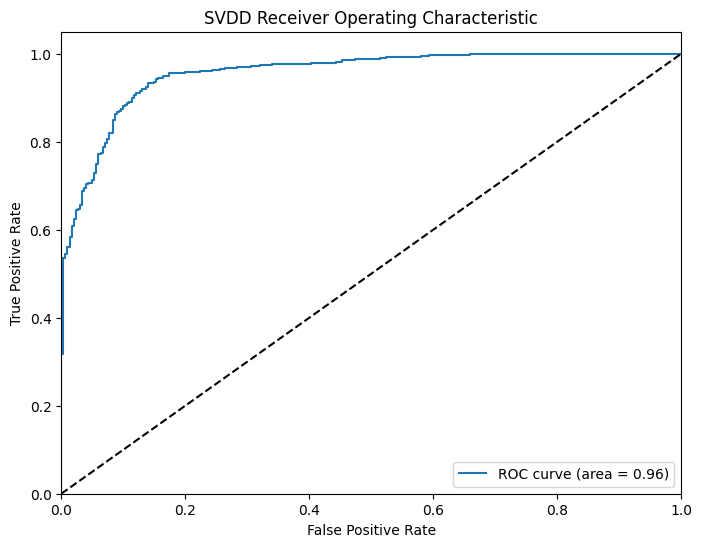
\includegraphics[width=0.45\textwidth]{Figures/svdd ROC.png}
        \label{fig:ROC SVDD}
    }
    \hspace{0.05\textwidth}
    \subfigure[ROC characteristics of the CAE model.]{
        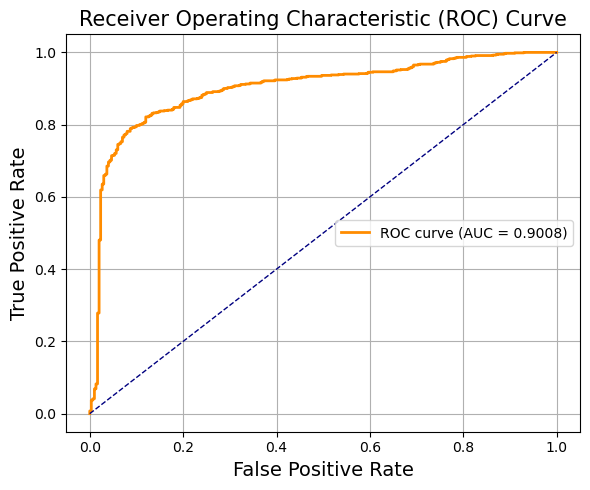
\includegraphics[width=0.4\textwidth]{Figures/ROC curve.png}
        \label{fig:ROC CAE}
    }
    \caption{Model performance.}
    \label{fig:Accuracy and loss plot}
\end{figure}

% Figure \ref{fig:ROC CAE} shows the ROC characteristics of the CAE model while Figure \ref{fig:ROC SVDD} shows the ROC characteristics of the SVDD Model. Overall, the performance of the model shows low false positive and false negative rates, which yields a good balance between precision and recall. This means that we are able to effectively detect anomalies while avoiding excessive false alarms.

% ---------- Results: ROC Analysis ----------

Figure~\ref{fig:ROC SVDD} depicts the the receiver–operating characteristic (ROC) of the
\textbf{Deep-SVDD} model, whereas Figure \ref{fig:ROC CAE} presents the ROC of the
\textbf{convolutional auto-encoder (CAE)}.
Both curves climb rapidly toward the upper-left corner, indicating low false–positive and false–negative
rates and, therefore, a favourable balance between precision and recall.
Closer inspection, however, reveals two nuances that match the quantitative findings in
Table~\ref{tab:cae_vs_svdd}:

\begin{itemize}
  \item \textbf{Steepness and stability (CAE, orange).}  
        The CAE ROC rises almost vertically and then hugs the left-hand axis,
        demonstrating robust discrimination across a broad range of operating
        thresholds.
        This geometry translates into a \textit{precision} of~$0.886$ and a
        \textit{recall} of~$0.906$ at the F$_1$-optimal decision boundary
        ($\text{threshold}=0.12$), yielding an $\text{AUC}=0.901$.
        Consequently, the CAE offers a generously wide ``safe zone’’ in which both
        Type-I and Type-II errors remain acceptably low—an attractive property for
        real-time deployment where threshold re-tuning is inevitable.

  \item \textbf{Higher plateau but concavity (SVDD, blue).}  
        Deep-SVDD attains a higher overall $\text{AUC}=0.955$, reflecting stronger
        rank-ordering ability.
        Nevertheless, its ROC exhibits a broader concave segment through the
        intermediate false-positive region, a signature of threshold instability.
        Numerically, this appears as a \textit{precision} of~$0.728$ despite
        perfect recall, implying that the model flags considerably more benign
        recordings as defective.
        From a decision-theoretic standpoint, such behaviour could lead to costly
        false alarms in an industrial monitoring scenario.
\end{itemize}

Taken together, the comparison shows that \textbf{Deep-SVDD excels in global ranking
(higher AUC), whereas the CAE delivers a more practical precision–recall trade-off
and greater threshold robustness}.
These observations align with the notebook’s per-epoch logs and the histogram of
reconstruction errors (Figure~\ref{fig:Reconstructed error plot}), corroborating that the CAE is the preferable choice when minimising false alarms is paramount, even if it
concedes a slight deficit in raw AUC.

The histogram of reconstruction errors presented in Figure \ref{fig:Reconstructed error plot} shows the separation between normal and anomalous instances. The distributions showed minimal overlap, with anomalous samples clustering toward higher error values. The 0.12 threshold clearly delineates the two classes.

\begin{figure}
    \centering
    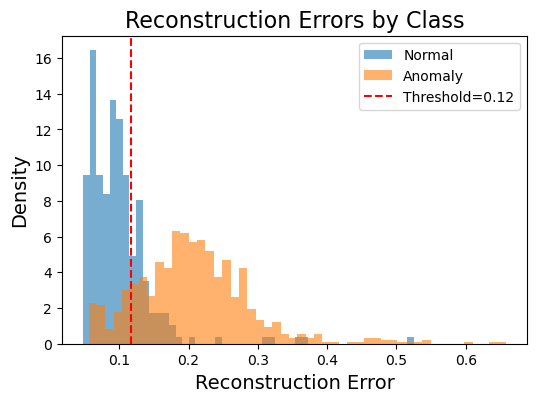
\includegraphics[width=0.8\linewidth]{Figures/Reconstruction error plot.png}
    \caption{Histogram over RMS values}
    \label{fig:Reconstructed error plot}
\end{figure}